\subsection{Solución actividad 4}

\subsubsection{Sistema 1}

Código en Matlab:

\begin{lstlisting}[language=Matlab]
x=0:10:620;
y= [32 33 34 36 38 39 40 40 40 40 39 39 39 37 37 38 38 38 38 38 38 39 38 38 38 38
38 38 38 38 38 38 38 38 38 38 38 38 38 38 38 38 38 38 38 38 38 38 38 38 38 38 38
38 38 38 38 38 38 38 38 38 38];

z= [1.6 1.7 1.8 1.9 2 2.1 2.17 2.135 2.137 2.328 2.117 2.103 2.094 1.95
1.98 2 2 2.01 2.07 2.067 2.065 2.085 2.07 2.067 2.065 2.064 2.062 2.06
2 2.056 2.055 2.052 2.05 2.048 2.05 2.052 2.055 2.055 2.055 2.049 
2.057 2.058 2.058 2.061 2.062 2.061 2.061 2.06 2.058 2.058 2.054
2.052 2.05 2.048 2.047 2.058 2.058 2.058 2.06 2.06
2.06 2.06 2.06];

plot(x,y,'b')
ylabel('Temperatura [c]')
xlabel('Tiempo [s]')
grid on

plot(x,z,'r')
ylabel('Voltaje [v]')
xlabel('Tiempo [s]')
grid on
\end{lstlisting}

Y ahora las gráficas anexadas como resultado del código.

\begin{figure}[H]
	\centering
	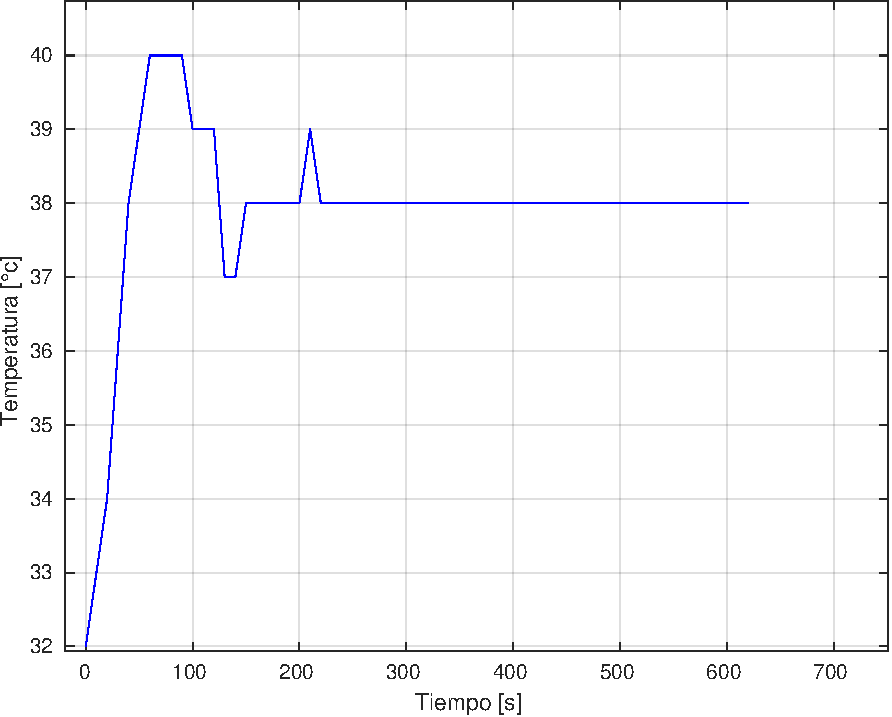
\includegraphics[width=0.7\linewidth]{img2/Grafica1}
	\caption{Gráfica de la temperatura vs tiempo}
	\label{fig:grafica1}
\end{figure}

\begin{figure}[H]
	\centering
	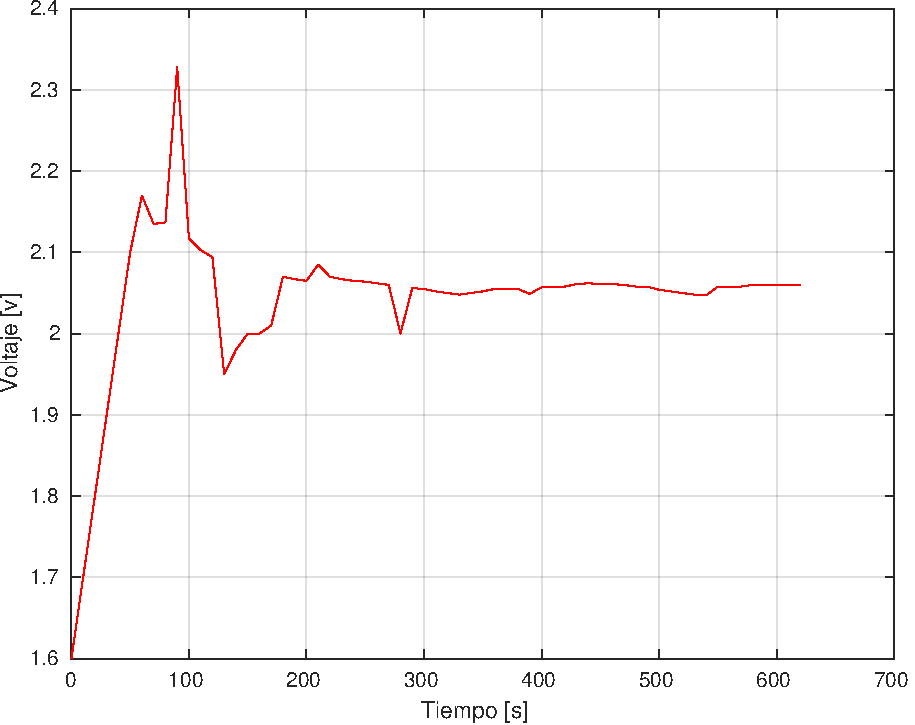
\includegraphics[width=0.7\linewidth]{img2/Grafica2}
	\caption{Gráfica del voltaje vs tiempo}
	\label{fig:grafica1}
\end{figure}

\textbf{3.-¿Cómo son las raíces del polinomio característicos del sistema de temperatura en estudio? justifique su respuesta.}

El comportamiento es sub-amortiguado, lo que quiere decir que primero tiene oscilaciones y después se estabiliza el sistema. $0<\zeta <1$ esta entre estos dos valores y por tanto las racies son complejas conjugadas de la forma:
$$-\zeta \omega_{n} \pm j \omega_{n} \sqrt{1-\zeta^{2}}$$

\textbf{4.-¿Las gráficas de voltaje y temperatura son continuas?}

Las gráficas son continuas, piense que la medición se usa tomando como eje x al tiempo y por tanto es continuo en ese eje. Si también se quiere decir que si la temperatura o el voltaje lo fueran, esto también se puede afirmar, ya que dichas mediciones su naturaleza es continua.
Como respuesta concreta, sí son continuas ambas gráficas.\\


\textbf{5.- ¿Cuál de las dos gráficas muestra mejor el comportamiento del sistema? Justifique su respuesta.}

La respuesta es algo subjetiva. Pienso que la gráfica de la temperatura muestra un mejor comportamiento sub-amortiguado, ya que las variaciones  para estabilizarse son menores y más predecibles que las variaciones del voltaje.


